\documentclass[../../../main.tex]{subfiles}

\begin{document}
    Das Verhalten der Laserleistung über die Zeit beim Einschaltvorgang ist in \ref{fig:Auswertung:6:Spikes} gezeigt. Beie Graphen zeigen beim Anstieg der Laserleistung die zu erwartenden Schwingungen. Verwunderlich ist, dass die Peaks der Spikes recht nahe oder sogar unter der stabilen Laserleistung nach dem Einschwingvorgang sind. Zu erwarten wären im Modell sehr starke Überschwingungen, die Abweichung davon lässt auf beachtliche Resonatorverluste schließen.\\

    Schließlich sei noch angemerkt, das der größere Injektionsstrom von $\SI{530}{\n\m}$ auch ein ausgeprägteres Spiking produziert. Dies ist plausibel, da ein höherer Injektionsstrom eine größere Pumpleistung bedingt, also schneller mehr Photonem im Nd:YAG-Kristall angeregt werden können. Daher kann eine höhere Besetzungsinversion erzeugt werden, bevor induzierte Emission von im Resonator umherfliegenden Photone einsetzt. Dies äußert sich in einer stärken Schwingung der Laserleistung.

    \begin{figure}[H]
        \centering
        \begin{subfigure}[b]{11cm}
            \centering
            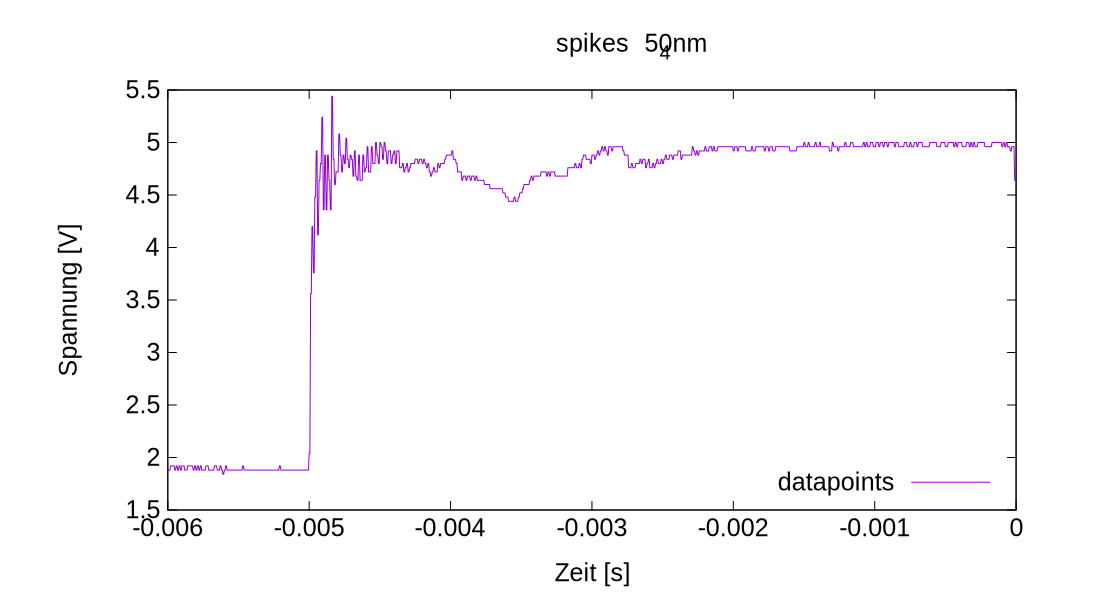
\includegraphics[width=\textwidth]{Bilddateien/6/spikes_450nm.png}
            \caption{Einschwingvorgang des Nd:YAG-Lasers bei einem Pumpstrom von $I_P = \SI{530}{\n\m}$}
            \label{fig:Auswertung:6:Spikes450nm}
        \end{subfigure}
        \hfill
        \begin{subfigure}[b]{11cm}
            \centering
            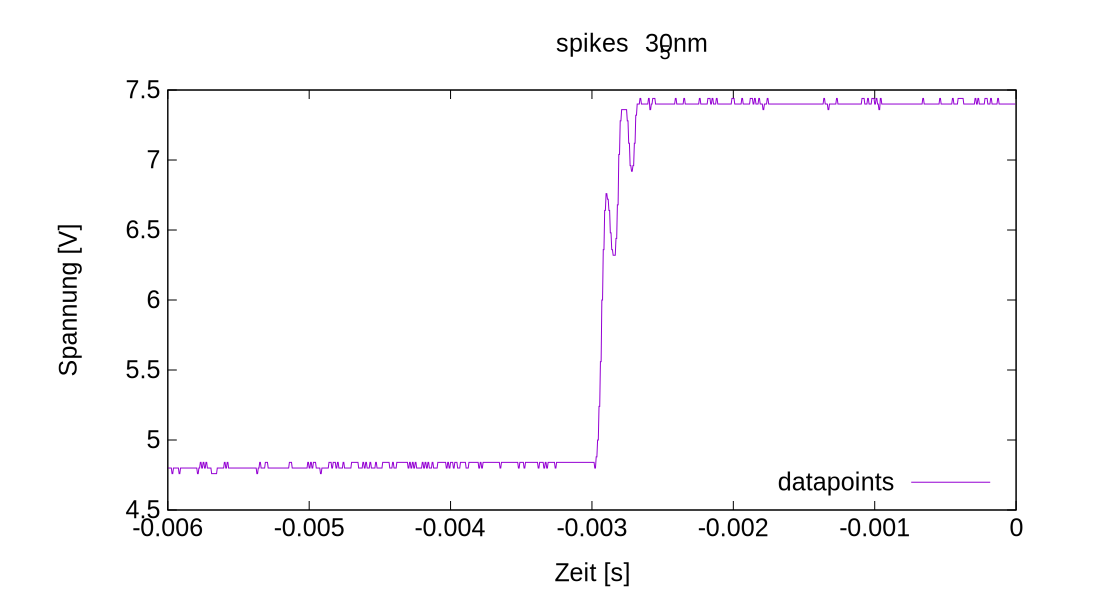
\includegraphics[width=\textwidth]{Bilddateien/6/spikes_530nm.png}
            \caption{Einschwingvorgang des Nd:YAG-Lasers bei einem Pumpstrom von $I_P = \SI{530}{\n\m}$}
            \label{fig:Auswertung:6:Spikes530nm}
        \end{subfigure}
        \caption{Zeitabhängige Laserleistung bei Beginn des Pumpens. Die Spannung auf der y-Achse beider Graphen korreliert direkt zu der Leistung der Lasers.}
        \label{fig:Auswertung:6:Spikes}
   \end{figure}

\end{document}